To write specifications for protocols' rich semantics, I employed ``interaction
tree'' (ITree), a generic data structure for representing interactive programs
in the Coq programming language, introduced by \citet{itree}.  I provide a brief
introduction to the ITree specification language in \autoref{sec:itree-lang}.

ITrees allow specifying protocols as monadic programs that model valid
implementations' possible behavior.  In \autoref{sec:qac-itree}, I show how to
embed specifications in the QAC family in terms of interaction trees.

The derivation from server specifications to interactive testers is by {\em
interpreting} ITree programs, which corresponds to the arrows
in \autoref{fig:framework}.  In \autoref{sec:interp}, I explain the mechanism of
interpretation by deriving testers from deterministic server models.  The rest
of this chapter then shows how to handle nondeterminism when interpreting
ITrees.

\subsection{Language definition}
\label{sec:itree-lang}
Consider an echo program, which keeps reading some data and writing it out
verbatim, until reaching EOF.  We can represent the program in Coq, with a
reference in C as:
\begin{multicols}{2}
\begin{coq}
  CoFixpoint echo :=
    c <- getchar;;
    if c is EOF
    then EXIT
    else
      putchar c;;
      echo.
\end{coq}
\columnbreak
\begin{cpp}
  void echo() {
    const char c = getchar();
    if (c == EOF)
      return;
    else {
      putchar(c);
      echo();
    }
\end{cpp}
\end{multicols}
Here the behavior after \ilc{getchar} depends on the value actually read.  The
monadic computation in Coq can be desugared into:
\begin{coq}
  CoFixpoint echo :=
    Bind getchar
         (fun c => if c is EOF
                 then EXIT
                 else Bind (putchar c)
                           (fun _ => echo)
         ).
\end{coq}
Such continuation-passing style can be represented as a tree of interactions.
To help readers better understand the interaction tree language, I first provide
a modified version of it that better shows its tree structure, and then explain
the actual type definition used in practice.

\begin{figure}
\begin{coq}
  CoInductive itreeM (E: Type -> Type) (R: Type) :=
    Ret     : R   -> itreeM E R
  | Trigger : E R -> itreeM E R
  | Bind    : forall {X : Type}, itreeM E X -> (X -> itreeM E R) -> itreeM E R.
\end{coq}
\caption{Mock definition of interaction trees.}
\label{fig:mock-itree}
\end{figure}

\begin{figure}
  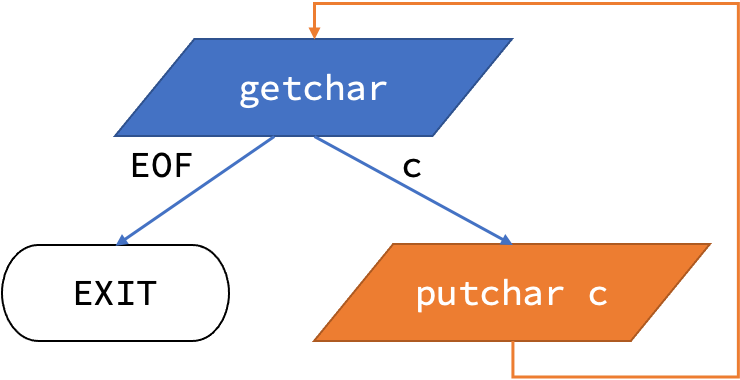
\includegraphics[width=.5\linewidth]{figures/echo-itree}
  \caption{Interaction tree for echo program}
  \label{fig:echo-itree}
\end{figure}

\paragraph{Mock interaction trees}
As shown in \autoref{fig:mock-itree}, a mock interaction tree (\ilc{itreeM}) has
two kinds of leaves, \ilc{Ret} and \ilc{Trigger}, and has internal nodes
constructed by \ilc{Bind}:
\begin{itemize}
\item \ilc{(Ret r)} represents a pure computation that yields a value \ilc r.
  In the echo example, \ilc{EXIT} halts the program with return value zero:
\begin{coq}
  Definition EXIT := Ret 0.
\end{coq}

\item \ilc{(Trigger e)} performs an impure event \ilc e and returns its result.
  Here \ilc{(e: E R)} is an event whose result is of type \ilc R.  For example,
  \ilc{getchar} has result type \ilc{char}, and \ilc{putchar}'s result type is
  \ilc{unit} (which corresponds to \inlinec{void} in C/C++, or \ilc{()} in
  Haskell).  These effective programs are constructed by triggering standard I/O
  events:
\begin{coq}
  Variant stdioE: Type -> Type := (* event type *)
    GetChar:         stdioE char
  | PutChar: char -> stdioE unit.
  
  Definition getchar           : itreeM stdioE char := Trigger  GetChar.
  Definition putchar (c: char) : itreeM stdioE unit := Trigger (PutChar c).
\end{coq}
\item \ilc{(Bind m k)} binds the return value of \ilc m to the continuation
  function \ilc k.  It first runs program \ilc m until it returns some value of
  type \ilc X.  The return value \ilc{(x: X)} then instantiates \ilc k into the
  following computation \ilc{(k x: itreeM E R)}.  This corresponds to the
  monadic \ilc{(;;)} syntax:
\begin{coq}
  Notation "x <- m1;; m2" := (Bind m1 (fun x => m2)).
  Notation "m1;; m2"      := (Bind m1 (fun _ => m2)).
\end{coq}

As illustrated in \autoref{fig:echo-itree}, each possible return value \ilc x is
an edge that leads to the child it instantiates, {\it i.e.}, \ilc{(k x)}.  In this
way, the \ilc{Ret} and \ilc{Trigger} nodes are connected into a tree
structure.
\end{itemize}

The mock interaction tree provides an intuitive continuation-passing structure
for representing impure programs.  However, to implement dualization
effectively, we need to revise the language definition of monadic binding.

\paragraph{Practical interaction trees}

\begin{figure}
\begin{coq}
  CoInductive itree (E: Type -> Type) (R: Type) :=
    Pure   : R -> itree E R
  | Impure : forall {X : Type}, E X -> (X -> itree E R) -> itree E R.
\end{coq}
\caption{Formal definition of interaction trees (simplified)}
\label{fig:itrees}
\end{figure}

Instead of binding a program to a continuation, ITree binds a single impure
event, as shown in \autoref{fig:itrees}.  I use \ilc{(Impure e k)} to
replace \ilc{(Bind (Trigger e) k)} representations in \ilc{itreeM}.
A \ilc{Pure} computation cannot be bound to a continuation, and must be the leaf
of an ITree.\footnote{For readability, the ``practical'' ITree definition is a
simplified version from \citet{itree}.  Here \ilc{Pure} and \ilc{Impure}
correspond to the \ilc{Ret} and \ilc{Vis} constructors.  I dropped the \ilc{(Tau
: itree E R -> itree E R)} constructor, which carries no semantics and is used
for satisfying Coq's guardedness condition.}

The \ilc{Ret}, \ilc{Trigger}, and \ilc{Bind} constructors introduced in
\ilc{itreeM} have equivalent representations in \ilc{itree}, so we can still
write programs in the monadic syntax:
\begin{coq}
  Definition ret {E R} : R -> itree E R := Pure.
  
  Definition trigger {E R} (e: E R) : itree E R := Impure e Pure.

  CoFixpoint bind {X E R} (m: itree E X) (f: X -> itree E R) : itree E R :=
    match m with
    | Pure   x   => f x
    | Impure e k => Impure e (fun r => bind (k r) f)
    end.

  Notation "x <- m1;; m2" := (bind m1 (fun x => m2)).
  Notation "m1;; m2"      := (bind m1 (fun _ => m2)).

  CoFixpoint translateM {E R} (m: itreeM E R) : itree E R :=
    match m with
    | Ret     r => ret r
    | Trigger e => trigger e
    | Bind m1 k => x <- translateM m1;; translateM (k x)
    end.
\end{coq}

\subsection{QAC in ITrees}
\label{sec:qac-itree}
The ITree specification language is a superset of the QAC language family.  Any
server model in \autoref{sec:qac-model} can be translated into an interaction
tree that receives requests and sends responses.

The deterministic server's event type is defined as follows:
\begin{coq}
  Variant ioE (I O: Type) : Type -> Type := (* I/O event *)
    Recv: qaE I                     (* receive an input  *)
  | Send: O -> qaE unit.            (* send    an output *)

  Definition qaE := ioE Q A.
\end{coq}
Here \ilc{ioE} is a parameterized event that takes types \ilc I and \ilc O as
arguments.  Type \ilc{qaE} is an instance of I/O event that receives requests of
type \ilc Q and sends responses of type \ilc A.

Given a loop body \ilc{sstep} and an initial state \ilc s, we can define the
interaction tree of the server model as a recursive program:
\begin{coq}
  CoFixpoint detServer (sstep: Q -> sigma -> A * sigma) (s: sigma) : itree qaE void :=
    q <- trigger Recv;;
    let (a, s') := sstep q s in
    trigger (Send a);;
    detServer sstep s'.
\end{coq}
The server program iterates over state \ilc{(s: sigma)}.  In each iteration, it
receives a request \ilc{(q: Q)} and computes the response \ilc{(a: A)} using the
state monad function \ilc{sstep}.  It then sends back the response and recurses
with the post state \ilc{(s': sigma)}.

To specify a nondeterministic server with internal choices of type $C$, I
introduce another event to represent its internal choices.
\begin{coq}
  Variant choiceE: Type -> Type :=
    Choice: choiceE C.    (* make an internal choice *)

  Definition qacE: Type -> Type := qaE +' choiceE.
\end{coq}
Here \ilc{qacE} is a sum type of \ilc{qaE} and \ilc{choiceE} events, meaning
that the server's events are either sending/receiving messages or making
internal choices.

At the beginning of each iteration, the nondeterministic server makes an
internal choice \ilc{(c: C)} as the seed of its \ilc{sstep} function:
\begin{coq}
  CoFixpoint server (sstep: Q -> C -> sigma -> A * sigma) (s: sigma) : itree qacE void :=
    c <- trigger Choice;;
    q <- trigger Recv;;
    let (a, s') := sstep q c s in
    trigger (Send a);;
    server sstep s'.
\end{coq}

Such server models can be derived into tester programs by interpretation.

\subsection{Interpreting interaction trees}
\label{sec:interp}
To interpret an ITree is to specify the operational semantics of its events.
For example, the \ilc{tester} program in \autoref{sec:interactive-testing} can
be constructed by interpreting a deterministic server model in
\autoref{sec:qac-itree}.

\paragraph{Tester event type}
An interactive tester generates requests and sends them to the SUT, receives
responses, and validates its observation against the specification:
\begin{coq}
  Variant genE: Type -> Type :=
    Gen : genE Q.          (* generate a request *)

  Variant exceptE: Type -> Type :=
    Throw: forall X, exceptE X. (* throw an exception *)

  Definition testE := ioE A Q +' genE +' exceptE.
\end{coq}
This type definition is pronounced as: ``The tester receives responses \ilc A as
input, sends requests \ilc Q as output, generates requests to send, or throws an
exception when it detects a violation in its observations.

\paragraph{Dualizing server events}
The tester is constructed by dualizing the server specification's behavior: When
the specification receives a request, the tester generates a request and sends
it to the SUT; When the specification sends a response, the tester expects to
receive the response from the SUT.  We can write this correspondence as a
function from server events to the tester's behaviors:
\begin{coq}
  Definition dualize {R} (e: qaE R) : itree testE R :=
    match e with
    | Recv   => q <- trigger Gen;;
                trigger (Send q);;
                ret q
    | Send a => a' <- trigger Recv;;
                if a' =? a
                then ret tt
                else trigger (Throw ("Expect " ++ a ++ " but observed " ++ a'))
    end.
\end{coq}
The \ilc{dualize} function takes an event and yields an ITree program.  It maps
the server's receive event to the tester's generate and send operations, and
vice versa, maps the server's send event to the tester's receive operation.  If
the tester's received response differs from that specified by the server model,
then the tester throws an exception to indicate a violation it detected.

\paragraph{Applying event handlers}
The \ilc{dualize} function is also called a handler.  It produces an ITree that
has the same result type as its argument event.  Therefore, we can construct the
tester by substituting the server's events with the operations defined by the
handler function:
\begin{coq}
  CoFixpoint interp {E F T} (handler: forall {R}, E R -> itree F R) (m: itree E T)
             : itree F T :=
    match m with
    | Pure   r   => Pure r
    | Impure e k => x <- f e;;
                    interp handler (k x)
    end.

  Definition tester (sstep: Q -> sigma -> A * sigma) (s: sigma) : itree testE void :=
    interp dualize (detServer sstep s).
\end{coq}
Applying the dualization handler to the server model gives us an ITree program
that performs tester interactions.  The tester keeps generating, sending and
receiving messages until observing an unexpected response when it throws an
exception and rejects the SUT.  It is semantically equivalent to the
\ilc{tester} in \autoref{sec:interactive-testing}.

To derive testers from nondeterministic server models, I design more complex
tester events and handlers, as discussed in the following sections.
